%%%%%%%%%%%%%%%%%%%%%%%%%%%%%%%%%%%%%%%%%%%%%%%%%%%%%%%%%%%%%%%%%%%%%%%%%%%%%
%%% LaTeX-Rahmen fuer das Erstellen von Diplomarbeiten
%%%%%%%%%%%%%%%%%%%%%%%%%%%%%%%%%%%%%%%%%%%%%%%%%%%%%%%%%%%%%%%%%%%%%%%%%%%%%

%%%%%%%%%%%%%%%%%%%%%%%%%%%%%%%%%%%%%%%%%%%%%%%%%%%%%%%%%%%%%%%%%%%%%%%%%%%%%
%%% allgemeine Einstellungen
%%%%%%%%%%%%%%%%%%%%%%%%%%%%%%%%%%%%%%%%%%%%%%%%%%%%%%%%%%%%%%%%%%%%%%%%%%%%%

\documentclass[twoside,12pt,a4paper]{report}
%\usepackage{reportpage}
\usepackage{epsf}
\usepackage{graphics, graphicx}
\usepackage{latexsym}
\usepackage{amsfonts}
\usepackage{amsmath}
\usepackage{listings}
\usepackage{url}
\usepackage{textcomp}
\usepackage[numbers]{natbib}
\usepackage[margin=10pt,font=small,labelfont=bf]{caption}
\usepackage[utf8]{inputenc}

\usepackage{xcolor}
\usepackage{hyperref}
\definecolor{darkred}{rgb}{0.5,0,0}
\definecolor{red}{rgb}{1,0,0}
\definecolor{darkgreen}{rgb}{0,0.5,0}
\definecolor{darkblue}{rgb}{0,0,0.5}
\definecolor{gray}{gray}{.6}

\definecolor{javared}{rgb}{0.6,0,0} % for strings
\definecolor{javagreen}{rgb}{0.25,0.5,0.35} % comments
\definecolor{javapurple}{rgb}{0.5,0,0.35} % keywords
\definecolor{javadocblue}{rgb}{0.25,0.35,0.75} % javadoc


%\lstloadlanguages{Java,XML,HTML,C++,SQL,C}
\hypersetup{colorlinks,
linkcolor=darkblue,
citecolor=darkgreen,
urlcolor=blue
}

%\lstdefinelanguage[GNU99]{Ruby}


\lstloadlanguages{RUBY} 
 \lstset{ 
  language=RUBY, 
  numbers=left, 
  numberstyle=\footnotesize, 
  numbersep=5pt, 
  tabsize=2, 
  breaklines=true, 
  frame=tb, 
  basicstyle=\ttfamily\scriptsize\small, 
  keywordstyle=\bfseries\itshape\color{javadocblue}, 
  morekeywords={puts, loop, defined, lambda, where}, 
  commentstyle=\color{gray}, 
  stringstyle=\color{javared}, 
  showspaces=false, 
  showstringspaces=false, 
  backgroundcolor=\color{white}, 
  title=\lstname 
  }
  

\textwidth 14cm
\textheight 22cm
\topmargin 0.0cm
\evensidemargin 1cm
\oddsidemargin 1cm
%\footskip 2cm
\parskip0.5explus0.1exminus0.1ex

% Kann von Student auch nach pers\"onlichem Geschmack ver\"andert werden.
\pagestyle{headings}

\sloppy

\begin{document}

%%%%%%%%%%%%%%%%%%%%%%%%%%%%%%%%%%%%%%%%%%%%%%%%%%%%%%%%%%%%%%%%%%%%%%%%%%%%
%%% hier steht die neue Titelseite 
%%%%%%%%%%%%%%%%%%%%%%%%%%%%%%%%%%%%%%%%%%%%%%%%%%%%%%%%%%%%%%%%%%%%%%%%%%%%
 
\begin{titlepage}
 \begin{center}
  {\LARGE Eberhard Karls Universit\"at T\"ubingen}\\
  {\large Mathematisch-Naturwissenschaftliche Fakultät \\
Wilhelm-Schickard-Institut f\"ur Informatik\\[4cm]}
  {\huge Diplom Thesis Informatics\\[2cm]}
  {\Large\bf  Mit der Trello-API rummuckeln\\[1.5cm]}
 {\large Sebastian Engel}\\[0.5cm]
24th July 2012\\[4cm]
{\small\bf Referees}\\[0.5cm]
  \parbox{7cm}{\begin{center}{\large Name Erstgutachter}\\
   (Bioinformatik)\\
  {\footnotesize Wilhelm-Schickard-Institut f\"ur Informatik\\
	Universit\"at T\"ubingen}\end{center}}\hfill\parbox{7cm}{\begin{center}
  {\large Name Zweitgutachter}\\
  (Biologie/Medizin)\\
  {\footnotesize Medizinische Fakult\"at\\
	Universit\"at T\"ubingen}\end{center}
 }
  \end{center}
\end{titlepage}

%%%%%%%%%%%%%%%%%%%%%%%%%%%%%%%%%%%%%%%%%%%%%%%%%%%%%%%%%%%%%%%%%%%%%%%%%%%%
%%% Titelr"uckseite: Bibliographische Angaben
%%%%%%%%%%%%%%%%%%%%%%%%%%%%%%%%%%%%%%%%%%%%%%%%%%%%%%%%%%%%%%%%%%%%%%%%%%%%

\thispagestyle{empty}
\vspace*{\fill}
\begin{minipage}{11.2cm}
\textbf{Engel, Sebastian:}\\
\emph{Titel der Arbeit}\\ Diplom Thesis Bioinformatics\\
Eberhard Karls Universit\"at T\"ubingen\\
Thesis period: 13th march to 11th September 2012
\end{minipage}
\newpage

%%%%%%%%%%%%%%%%%%%%%%%%%%%%%%%%%%%%%%%%%%%%%%%%%%%%%%%%%%%%%%%%%%%%%%%%%%%%

\pagenumbering{roman}
\setcounter{page}{1}

%%%%%%%%%%%%%%%%%%%%%%%%%%%%%%%%%%%%%%%%%%%%%%%%%%%%%%%%%%%%%%%%%%%%%%%%%%%%
%%% Seite I: Zusammenfassug, Danksagung
%%%%%%%%%%%%%%%%%%%%%%%%%%%%%%%%%%%%%%%%%%%%%%%%%%%%%%%%%%%%%%%%%%%%%%%%%%%%


\section*{Abstract}

Trello is a collaboration webservice to manage projects and assign their todo items to co-workers. There are many collaboration tools today, but most of them are very basic. Trello is very extensive and it is optimal fo small businesses. But although it works fine like it's supposed to it has its limits. Trello as its state now is a closed system. Nothing gets in or out unless you use Trello itself. But sometimes it would be handy if you were able to get content from Trello out into other applications. For example a CMS which should contain completed theses which you are already managing in Trello.
 
So this thesis addresses small scripts which let Trello interact with other webservices and applications. For this purpose I wrote a wrapper of the Trello API in Ruby to accomplish this task in the most dynamic way possible.
\newpage
\section*{Acknowledgements}

Write here your acknowledgements.

\cleardoublepage

%%%%%%%%%%%%%%%%%%%%%%%%%%%%%%%%%%%%%%%%%%%%%%%%%%%%%%%%%%%%%%%%%%%%%%%%%%%%%
%%% Table of Contents
%%%%%%%%%%%%%%%%%%%%%%%%%%%%%%%%%%%%%%%%%%%%%%%%%%%%%%%%%%%%%%%%%%%%%%%%%%%%%

\renewcommand{\baselinestretch}{1.3}
\small\normalsize

\tableofcontents

\renewcommand{\baselinestretch}{1}
\small\normalsize

\cleardoublepage

%%%%%%%%%%%%%%%%%%%%%%%%%%%%%%%%%%%%%%%%%%%%%%%%%%%%%%%%%%%%%%%%%%%%%%%%%%%%%
%%% List of Figures
%%%%%%%%%%%%%%%%%%%%%%%%%%%%%%%%%%%%%%%%%%%%%%%%%%%%%%%%%%%%%%%%%%%%%%%%%%%%%

\renewcommand{\baselinestretch}{1.3}
\small\normalsize

\addcontentsline{toc}{chapter}{List of Figures}
\listoffigures

\renewcommand{\baselinestretch}{1}
\small\normalsize

\cleardoublepage

%%%%%%%%%%%%%%%%%%%%%%%%%%%%%%%%%%%%%%%%%%%%%%%%%%%%%%%%%%%%%%%%%%%%%%%%%%%%%
%%% List of tables
%%%%%%%%%%%%%%%%%%%%%%%%%%%%%%%%%%%%%%%%%%%%%%%%%%%%%%%%%%%%%%%%%%%%%%%%%%%%%

\renewcommand{\baselinestretch}{1.3}
\small\normalsize

\addcontentsline{toc}{chapter}{List of Tables}
\listoftables

\renewcommand{\baselinestretch}{1}
\small\normalsize

\cleardoublepage

%%%%%%%%%%%%%%%%%%%%%%%%%%%%%%%%%%%%%%%%%%%%%%%%%%%%%%%%%%%%%%%%%%%%%%%%%%%%%
%%% List of abbreviations
%%%%%%%%%%%%%%%%%%%%%%%%%%%%%%%%%%%%%%%%%%%%%%%%%%%%%%%%%%%%%%%%%%%%%%%%%%%%%

% can be removed
\addcontentsline{toc}{chapter}{List of Abbreviations}
\chapter*{List of Abbreviations\markboth{LIST OF ABBREVIATIONS}{LIST OF ABBREVIATIONS}}

\begin{tabbing}
\textbf{FACTOTUM}\hspace{1cm}\=Schrott\kill
\textbf{BLAST}\>Basic Local Alignment Search Tool \\
\textbf{...} \> ...\\
\end{tabbing}

\cleardoublepage

%%%%%%%%%%%%%%%%%%%%%%%%%%%%%%%%%%%%%%%%%%%%%%%%%%%%%%%%%%%%%%%%%%%%%%%%%%%%%
%%% Der Haupttext, ab hier mit arabischer Numerierung
%%% Mit \input{dateiname} werden die Datei `dateiname' eingebunden
%%%%%%%%%%%%%%%%%%%%%%%%%%%%%%%%%%%%%%%%%%%%%%%%%%%%%%%%%%%%%%%%%%%%%%%%%%%%%

\pagenumbering{arabic}
\setcounter{page}{1}

%% Introduction
%%%%%%%%%%%%%%%%%%%%%%%%%%%%%%%%%%%%%%%%%%%%%%%%%%%%%%%%%%%%%%%%%%%%
% Einleitung
%%%%%%%%%%%%%%%%%%%%%%%%%%%%%%%%%%%%%%%%%%%%%%%%%%%%%%%%%%%%%%%%%%%%

\chapter{Introduction}\label{Introduction}

Blablabla.....

\medskip
Die Arbeit gliedert sich dazu wie folgt: Die Grundlagen von BlaBlaBla 
werden in Kapitel~\ref{Introduction} erarbeitet. 
...
Eine
Diskussion und ein kurzer Ausblick im
Kapitel~\ref{Discussion} beschlie\"sen diese Arbeit.

Bevor wir uns der Auswertung bzw. Bewertung der gewonnenen Prim\"ardaten zuwenden, wollen wir zun\"achst einige grundlegende Begriffe der deskriptiven Statistik wiederholen.


\cleardoublepage

%% 
%%%%%%%%%%%%%%%%%%%%%%%%%%%%%%%%%%%%%%%%%%%%%%%%%%%%%%%%%%%%%%%%%%%%
% Grundlagen
%%%%%%%%%%%%%%%%%%%%%%%%%%%%%%%%%%%%%%%%%%%%%%%%%%%%%%%%%%%%%%%%%%%%

\chapter{Principles}
  \label{Principles}

\section{Trello}

\subsection{How Trello works}\index{Trello}
Trello is a webservice by the New York City based web corporation Fog Creek Software\footnote{Official Fog Creek Software website: \url{http://www.fogcreek.com}}\index{Fog Creek Software}. It is a collaboration tool to manage projects, launched in 2011\footnote{The original launch post in the Trello blog: \url{http://blog.trello.com/launch/}}. 

\begin{figure}[htb]
\centering
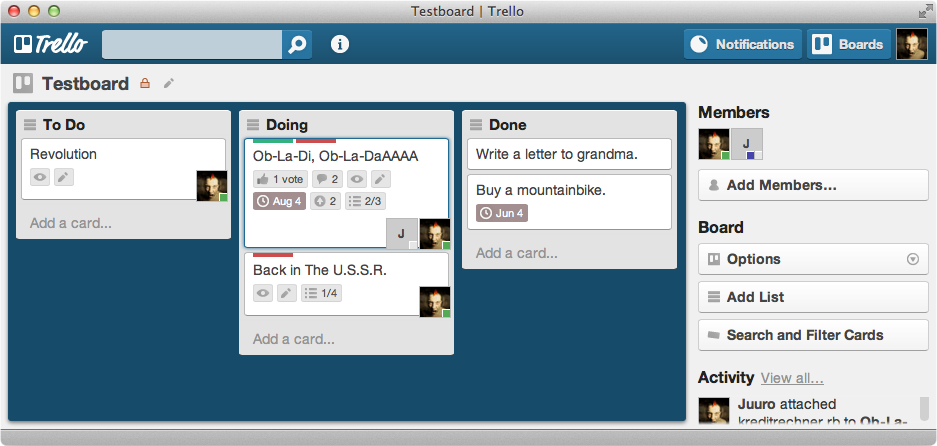
\includegraphics[width=\textwidth]{figures/trello}
\caption{A Trello board.}
\label{fig:trello}
\end{figure}

There is the concept of so called \emph{boards} which contents several configurable lists. Figure \ref{fig:trello} shows a board with the three standard lists \emph{To Do}, \emph{Doing} and \emph{Done}. In these lists the user can create todo items. These todo items are called \emph{cards}. The cards can contain several additional data. Each card has a title and maybe a description, some asigned members, a due date, some labels, votes, checklists, comments and attachments. The creator of the board is the owner in the first place and the owner can add other Trello users to his boards and cards. So everone who's working on a project can see whats going on at the moment. Users who are assigned to a board can even create new todo items by themselves. If somebody works at more than one company with many projects each there is the concept of \emph{organizations}. This is useful in order to ensure a clear separation.

\begin{figure}[htb]
\centering
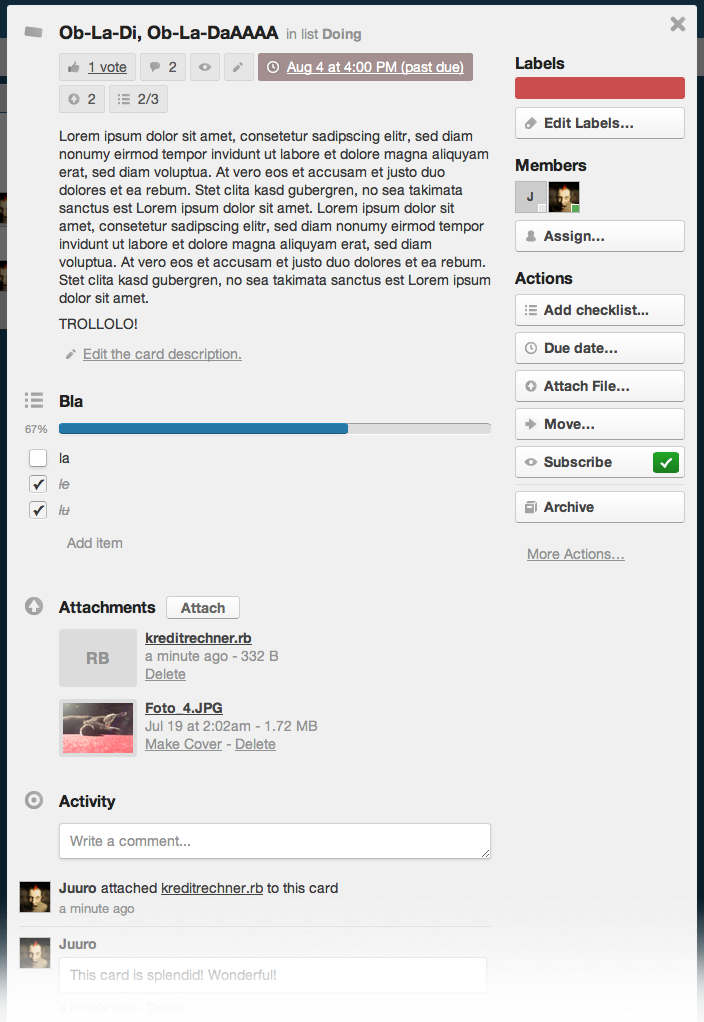
\includegraphics[width=\textwidth]{figures/trello-card}
\caption{A opened card in Trello.}
\label{fig:trello-card}
\end{figure}

\subsection{Why Trello}\index{Trello}
Trello is not just one of hundreds of thousands of todo applications. It is streamlined for the purposes of small businesses. So for the needs in the university with small groups of people working on the same things it is perfect. Trello has proofed its value several months already. The Trello website is written in HTML 5\index{HTML!5} with the use of AJAX\index{AJAX} where it makes sense. Trello provides an iOS\index{iOS} \cite{trello:ios} and Android\index{Android} \cite{trello:android} app. Both are constantly evolving. So the system is state-of-the-art. In addition the company behind Trello is not just a start-up with three employees. Thats important, too. A product of a small business, which is based just on the enthusiasm of the founders often doesn't last long. Fog Creek Software is over ten years old and has several products.

The first wish was to see the due dates of the cards anybody is assigned to in Google Calendar. But thinking about that there were many other use cases for small scripts which could run as cron jobs on a server to serve several regular tasks. These scripts are described in more detail in Chapter 3.

\subsection{Trello API}\index{API}
Trello has an API \nomenclature{API}{Application Programming Interface} which is still in beta at the moment I'm writing this. But it is already very extensive. \cite{trello:docu}

\subsubsection{Authentification}
Though the scripts which are used here need access to private boards in Trello\index{Trello} there has to be any kind of authentification. For user applications with a frontend the Trello API provides OAuth2. But because of the concept of OAuth2 the user is required to enter his Trello username and password. \cite{oauth} My scripts are supposed to run on servers as cron jobs. There is no user who could manually enter data. For this kind of applications Trello provides a key/token-system. Every user has a private key. Whith this key the user can generate a token. This token will be send along every request to the Trello API. The token tells Trello which scope the request can see. While generating a token one can specify the scope of the token and when it will expire. The possible expriations of a token are between one day and never. In our case we will use \emph{never}. To generate a token one has to visit a special URL:
\texttt{
https://trello.com/1/authorize?key=SUBSTITUTEWITHYOURPRIVATEKEY \&name=My+Application\&expiration=never\&response\_type=token \&scope=read,write}
In this example the token would never expire and could read and write everything the user can access with the API. Other valid values instead of \texttt{never} for expiration would be \texttt{1day}, \texttt{30days}. \texttt{30days} is the default value. \cite{trello:gettingstarted}

\subsubsection{REST}\nomenclature{REST}{Representational State Transfer}
The Trello API is a \emph{RESTful} web API. That means that the API is conform to the REST design model. REST is a common style of software architecture for distributed systems. It's built on four of the HTTP request methods: GET, POST, PUT and DELETE. An implementation of a REST web service follows four basic design principles:
\begin{itemize}
	\item Use HTTP\nomenclature{HTTP}{Hyper Text Transfer Protocol} methods explicitly.
	\item Be stateless.
	\item Expose directory structure-like URIs\nomenclature{URI}{Uniform Resource Identifier}.
	\item Transfer XML\nomenclature{XML}{Extensible Markup Language} , JSON\nomenclature{JSON}{JavaScript Object Notation}, or both.
\end{itemize}
\cite{rest}

Following these conventions a GET URL of a RESTful web service looks like this:
\begin{center}
\texttt{https://api.trello.com/1/cards/4fc8dd3e1b9ecf0c3571902f? key='PRIVATEKEY\&token=TOKEN}
\end{center}
This is a GET request to get a specific card with the id \texttt{4fc8dd3e1b9ecf0c3571902f}. If this URL\nomenclature{URL}{Uniform Resource Locator} is visited in a browser (with correct \emph{key} and \emph{token}) the browser will show plain JSON. In order Ruby can work with it, it must be able to capture this data somehow. To fulfil the requirements of REST in Ruby there are several gems. Here the RestClient gem is used. This GET request with the RestClient gem in Ruby looks like \ref{listing019}.

\begin{lstlisting}[aboveskip=1\baselineskip, caption=GET request using RestClient., label=listing019]
member = RestClient.get('https://api.trello.com/1/cards/4fc8dd3e1b9ecf0c3571902f?key='+$key+'&token='+$token)
pp JSON.parse(member)
\end{lstlisting}

In comparison to the open-uri library, which is included in the Ruby standard library, it's much more tidied up when it comes to POST requests.

\begin{lstlisting}[aboveskip=1\baselineskip, caption=POST request using RestClient., label=listing009]
response = RestClient.post(
	'https://api.trello.com/1/boards',
	:name => board['name'], 
	:desc => board['desc'],
	:key => $key,
	:token => $token
)
\end{lstlisting}

\begin{lstlisting}[aboveskip=1\baselineskip, caption=POST request with open-uri., label=listing010]
uri = URI('https://api.trello.com/1/boards')
req = Net::HTTP::Post.new(uri.path)

req.set_form_data(
	'name' => board['name'], 
	'desc' => board['desc'],
	'key'=>$key,
	'token'=>$token
)

Net::HTTP.start(uri.host, uri.port, :use_ssl => uri.scheme == 'https') do |http|
	response = http.request(req)
end
\end{lstlisting}

Listing \ref{listing009} and listing \ref{listing010} show the very same API call. But \ref{listing009} is realised with RestClient and listing \ref{listing010} with open-uri. Not even is the open-uri code much longer, but open-uri doesn't detect the correct scheme from the given URI. If the call should performed in HTTPS this has to be set explicitly. That implies that for the handling of RESTful web services RestClient is the better choice.


\section{Ruby}\index{Ruby}
Ruby is a modern general-purpose object-oriented programming language. Its big difference to most other languages is that it focuses on humans rather than computers. 

Yukihiro Matsumoto, the designer of Ruby, said once:
\begin{quote}
Ruby is simple in appearance, but is very
complex inside, just like our human body.\cite{ruby:talk}
\end{quote}

That means, that Ruby\index{Ruby} is very easy readable and is intuitive for humans even so it can perform complex tasks. This is achieved with English keywords instead of brackets and curly brackets. The result for the programmer of this consistent philosophy is a very easy to read language which is also very plain. Because of the English words instead of abstract characters Ruby is easy understandable. Even non-programmers understand mostly whats going on. So programmers produce way less errors while writing the code. A wrongly spelled word is more intuitive recognisable than a missing bracket or semicolon. \cite{ruby:about} More about Ruby can be found at \url{http://www.ruby-lang.org}.

\subsection{RubyGems}\index{RubyGems}
Ruby has a good amount of methods and classes every Ruby installation provides. But there are hundreds of extensions for special use cases – to communicate with RESTful Web APIs for example – made by third party developers. In Ruby such extensions are called \emph{gems}. To manage and publish these third party libraries theres is the standard \emph{RubyGems}. It provides a standard format for third party libraries for Ruby, a tool to manage the installation of gems and a server for distributing the gems. \cite{ruby:gemdev} Some Ruby distributions are delivered with several gems. Gems can be added to an existing Ruby installation at any time. 

To install an additional gem on a Unix operating system the following command can be used:  
\begin{center}
\texttt{gem install gemname}
\end{center}
Where \texttt{gemname} is the name of the respective gem. If the installation performed without errors, the gem is ready to use. \cite{ruby:gemdoc}

To use an installed gem in a Ruby\index{Ruby} script the following code at the top of the script before the code starts is necessary:

\begin{lstlisting}[aboveskip=1\baselineskip, caption=Using the gem \emph{gemname}, label=listing001]
require 'gemname'
\end{lstlisting}
Again, \emph{gemname} stands for the name of the respective gem. If any gems are used in these script which are not part of the Ruby standard library, they are listed at the beginning of the related description. Further information at \url{http://doc.rubygems.org} and \url{http://rubyforge.org/projects/rubygems/}.


\section{JSON}\index{JSON}
All the responses to Trello\index{Trello} API\index{API} calls use JSON\footnote{RFC\nomenclature{RFC}{Request For Comments} document for JSON: The application/json Media Type for JavaScript Object Notation (JSON)  \url{http://www.ietf.org/rfc/rfc4627.txt}}. It is a subset of the JavaScript programming language. Despite its relation to JavaScript it's language independent. JSON is da data-interchange format like XML. But JSON is built on two structures. One is a list of key/value pairs. In most programming languages this is realised as an hash, struct, object or associative array. The other structure is an ordered list of values. This is realised as array, list, vector or sequence in popular programming languages. In JSON itself these structures are called \emph{object} and \emph{array}. Objects start and end with curly brackets. Each key is followed by a colon and the key/value pairs are separated by commas. Arrays start and end with suqred brackets. The values are separated by commas. Both can be arbitrary nested. At every point one of my script saves content at any other place than Trello it's in the JSON\index{JSON} format, too. That's because it guarantees easy compatibility with Trello. JSON\index{JSON} can be saved in files, too. A JSON\index{JSON} file has the suffix \texttt{.json}. \cite{json}

\begin{lstlisting}[aboveskip=1\baselineskip, caption=JSON example., label=listing007]
{
    "id": "4eea4ffc91e31d1746000046",
    "name": "Example Board",
    "desc": "This board is used in the API examples",
    "lists": [{
        "id": "4eea4ffc91e31d174600004a",
        "name": "To Do Soon"
    }, {
        "id": "4eea4ffc91e31d174600004b",
        "name": "Doing"
    }, {
        "id": "4eea4ffc91e31d174600004c",
        "name": "Done"
    }]
}
\end{lstlisting}

In listing \ref{listing007} a JSON example is shown. This is the response of

\begin{center}
\texttt{https://api.trello.com/1/boards/4eea4ffc91e31d1746000046? lists=open\&list\_fields=name,desc\&key=PRIVATEKEY\&token=TOKEN}
\end{center}

The JSON in listing \ref{listing007} starts with a curly bracket. That means the uppermost structure is an object. Here are a few key/value pairs like \texttt{"id": "4eea4ffc91e31d1746000046"}. The key \texttt{"list"} has an array as value. So their value is in suqared brakets. Each element of the array is an object again.

To process the received JSON Ruby needs to parse it first. For that purpose there is the a gem simply called \emph{JSON}. It parses the JSON with the 

\begin{center}
\lstinline{JSON.parse(receivedJson)} 
\end{center}
command, where \lstinline{receivedJson} is a variable that contains the plain JSON received from the Trello API with a GET request. Aufter the parsing the JSOn objects are now represented as Ruby Hashes and the JSON arrays as Ruby arrays. To post content to the Trello API it has to be in JSON, too. So there is another method of the JSON class in Ruby which generates JSON from Ruby hashes and arrays. 

\begin{center}
\lstinline{JSON.generate(hashBoards)} 
\end{center}
\cleardoublepage

%%
%%%%%%%%%%%%%%%%%%%%%%%%%%%%%%%%%%%%%%%%%%%%%%%%%%%%%%%%%%%%%%%%%%%%
% Diskussion und Ausblick
%%%%%%%%%%%%%%%%%%%%%%%%%%%%%%%%%%%%%%%%%%%%%%%%%%%%%%%%%%%%%%%%%%%%
\onehalfspacing
\chapter{Applications}\label{applications}

\section{Export to HTML}\nomenclature{HTML}{Hyper Text Markup Language}\label{html.rb}

Used libraries:
\begin{itemize}
	\item \texttt{erb}
	\item \texttt{json}
	\item \texttt{rest\_client}
	\item \texttt{pp}
	\item \texttt{kramdown}
\end{itemize}

\begin{lstlisting}[aboveskip=1\baselineskip, style=bash, caption=\texttt{html.rb} usage., label=listing026]
ruby html.rb --title TITLE [-c CARDID[,CARDID]] [-l LISTID[,LISTID]] [-b BOARDID[,BOARDID]] [-a] [-t TOKEN] [-k KEY]
\end{lstlisting}

The \texttt{html.rb} script exports the data from one or more cards to an HTML file. The resulting HTML file lists the cards one below the other. The order is determined by the command-line argument. If the command-line looks like listing \ref{listing005}, the script will at first process the list with the id \texttt{4ffd78ff7f0c71780cc5aa1c}. That means that all cards in the list are in the HTML file and below these the single card with the id \texttt{4ffd78a2c063afeb066408b8}. In addition to the command-line options described in section \ref{cli}, the option \texttt{--title} is used. Here, the user has to specify a title for the web page. The title will be displayed at the top of the page in \lstinline{<h1>} HTML tags.

\begin{lstlisting}[aboveskip=1\baselineskip, style=bash, caption=Example of a \texttt{html.rb} call., label=listing005]
ruby html.rb -l 4ffd78ff7f0c71780cc5aa1c                 -c 4ffd78a2c063afeb066408b8 --title 'Madness'
\end{lstlisting} 

Each card is displayed with all its information. This includes title, description, members, due date, labels, votes, checklists, comments, and attachments.

Trello itself distinguishes between photos and other attachments. Normal attachments are linked under the description. Photos are embedded in the HTML code as thumbnails. Trello detects JPEG, GIF, and PNG files as pictures and displays them as thumbnails. In addition to these formats, the resulting HTML file displays TIFF, PSD, BMP, and JPEG2000 as thumbnails, too. All modern browsers support these formats.

The \texttt{html.rb} script generates static HTML. Of course, the requirements could also be met by a dynamic solution with PHP or Ruby on Rails. But the upside is that the user of the respective website doesn't have to wait for the webserver. Dynamic websites are mostly fast in the meantime, but with static HTML files, the developer is on the safe side. This approach pays off especially if the data to be displayed doesn't change every minute. The server doesn't have to generate the whole data with every visit. It just has to send the static HTML files.

\subsection{Markdown}\index{Markdown}
Markdown is a small lightweight plain text formatting snytax designed by John Gruber. It is designed for the use with blogs and CMS. In these cases, HTML is often too much. Markdown represents most of the features of HTML that are needed for writing. The designer of Markdown had the goal that a text, written in Markdown, is still easy to read. John Gruber provides a software tool written in the Perl programming language, that converts the Markdown formatted text to valid HTML. \cite{markdown}

\begin{lstlisting}[aboveskip=1\baselineskip, style=bash, caption=Example for a text written in Markdown., label=listing006]
### iCloud:(*@ \label{line002} @*)

1.   Shared Photo Streams Now you can *share* just the **photos** you want, with just the people you choose. (*@ \label{line003} @*)
2.   Reminder

------------------------------- (*@ \label{line004} @*)

Here is an example of AppleScript:

    tell application "Foo" (*@ \label{line005} @*)
        beep
    end tell

![Apple logo](http://upload.wikimedia.org/wikipedia/commons/f/fa/Apple_logo_black.svg "Apple logo") (*@ \label{line006} @*)
\end{lstlisting}


\begin{lstlisting}[aboveskip=1\baselineskip, style=html, caption=Listing \ref{listing006} converted to HTML., label=listing007]
<h3>iCloud:</h3>

<ol>
	<li>Shared Photo Streams Now you can <em>share</em> just the <strong>photos</strong> you want, with just the people you choose.</li>
	<li>Reminder</li>
</ol>

<hr>

<p>Here is an example of AppleScript:</p>

<pre>
	<code>tell application "Foo"
	beep
	end tell</code>
</pre>

<p><img alt="Apple logo" title="Apple logo" src="http://upload.wikimedia.org/wikipedia/commons/f/fa/Apple_logo_black.svg"></p>
\end{lstlisting} 

Listing \ref{listing006} shows a small example of Markdown. The \lstinline{###} in line \ref{line002} is a heading equal to \lstinline{<h3>} in HTML. The first list item of the ordered list in line \ref{line003} contains italic and bold words. In line \ref{line004}, there is a horizontal line. After a normal line of text, a code block starts in line \ref{line005}. At the end, in line \ref{line006}, there is a picture with \lstinline{title} and \lstinline{alt} texts. After the conversion, it looks like listing \ref{listing007} in HTML. The appearance, of course, depends on the used CSS on the respective websites. The appearance in Trello is as shown in figure \ref{fig:markdown-result}.

\begin{figure}[htb]
\centering
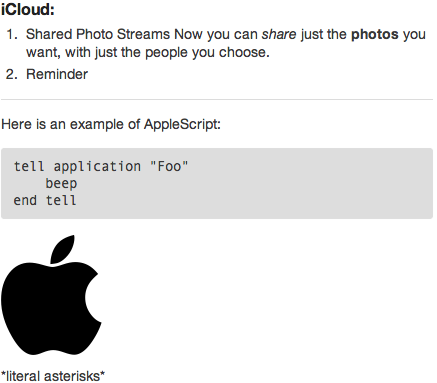
\includegraphics[scale=0.6]{figures/markdown-result}
\caption{The browser view of the HTML converted from the Markdown in listing \ref{listing006}}
\label{fig:markdown-result}
\end{figure}

Meanwhile, Markdown has become quite popular. Many blogging platforms support it, at least there are Markdown plug-ins for most platforms. Trello supports it in the description of cards. In the unlikely case that markdown reaches its limits, inline HTML can be used. The only restriction is that HTML block-level-elements have to be separated to the previous and following Markdwon blocks.

\subsubsection{kramdown}

In order to convert Markdown to HTML, the gem kramdown is used. Figure \ref{fig:kramdown} describes the convert options of kramdown. It converts HTML and Markdown to LaTeX, PDF, and a special kramdown format, too. The kramdown format is an extended Markdown syntax. Like input formats, it accepts HTML and kramdown besides standard Markdown. \cite{kramdown} These additional features might be useful for future approaches. To generate lists of bibliographies for scripts, papers or books.

\begin{figure}[htb]
\centering
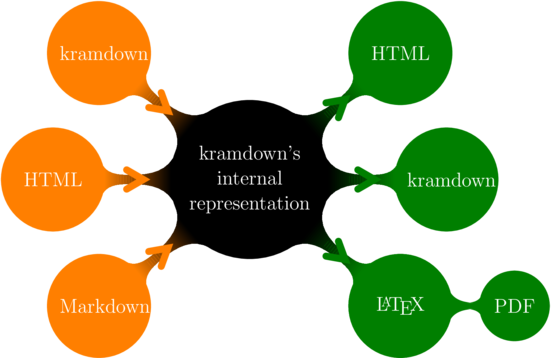
\includegraphics[width=\textwidth]{figures/kramdown}
\caption{Overview about kramdowns converting options. \cite{kramdown}}
\label{fig:kramdown}
\end{figure}

\subsection{Twitter Bootstrap Framework}\index{Twitter}\index{Bootstrap}
In 2011 Twitter released Bootstrap\footnote{Blog post form the lead developer about the launch of Twitter Bootstrap: \url{https://dev.twitter.com/blog/bootstrap-twitter}}. Bootstrap is a collection of methods and scripts for creating front-ends of websites. It contains templates for site structuring, tables, text, buttons, menus, forms, lists, and some other often used elements of websites. Additionaly, some functions are supported by JavaScript\index{JavaScript}. Bootstrap is written in HTML\index{HTML}, JavaScript, CSS\index{CSS}, and LESS\index{LESS}, which is a dynamic style sheet language and extension to CSS. This enables the use of variables, functions, nested selectors, and operators.\cite{less} Bootstrap is completely free of charge and under open source licence. \cite{bootstrap}

Bootstrap\index{Bootstrap} evolved at Twitter\index{Twitter} during work on several projects with different libraries. The projects became inconsistent and a high administrative effort was needed in order to maintain the site?. Some developers at Twitter led by Mark Otto worked on a tool to document and share common designs within the company. Twitter determined that this toolkit could be more than an intern helper tool. So they equipped it with all the common function which are needed for modern web development and released it on GitHub. \cite{markotto}

\subsection{HTML5}\index{HTML!5}
Twitter Bootstrap supports HTML5. HTML is the markup language for displaying content in a web browser. HTML5 is the latest revision of the HTML standard. It is an open format developed by the World Wide Web Consortium (W3C)\index{World Wide Web Consortium}\index{W3C}. HTML5 has been a working draft since 2008. In 2011, the HTML Working Group at W3C advanced HTML5 to Last Call. At the moment, HTML communities all over the world are asked to confirm the standard.  It is estimated that HTML5 will reach W3C Recommendation by 2014.\cite{html:lastcall} Although it is not yet finished, it is already widely used.

Before HTML5 there were two popular standards: HTML4\index{HTML!4} and XHTML1\index{XHTML}\nomenclature{XHTML}{Extensible Hyper Text Markup Language}. XHTML1 defines a XML\index{XML} serialisation for HTML4. With HTML5, there is only one language called HTML. This language can be written in HTML syntax and XML syntax. 
\cite{html:5differences} The W3C realised the importance of smartphones in the future early on. They guided the development of HTML5 with the consideration of being able to run on low-powered devices. The market share of HTML5 enabled devices is still rising. \cite{smartphonesales} Smartphone sales even beat PC sales in 2012. Thus, it is becoming increasingly important for web applications to work well on small devices. HTML5 is used to ensure this. The foundation created here can therefore be used as a basis for the future.

HTML5 introduces several new elements. Some of these are used in \texttt{html.rb}. At first, there is the \lstinline{<header>} element. A header is an area at the top of a web page. It is used for navigational aids, logos, or a search bar. \cite{html5:header} At the bottom is the \lstinline{<footer>} element, which can be used as a side wide footer and as a footer of sections. \cite{html5:footer} Here, it is just used as side wide footer as preparation for data like licencing information, imprint, and information about the author. The cards are enclosed in \lstinline{<article>} elements. Every single card is represented as an \lstinline{<article>} element. This makes sense because, typically, a card is an article, especially if the user would like the card to be displayed on a web page. The W3C requires an \lstinline{<article>} element to be self-contained. \cite{html5:article} A card is a collection of information which is ordered by the several types of data. 

This foundation of generating HTML out of Trello can be used in various ways. It is predestinated for websites with recurring kinds of information. Every business card style web page can definitely be managed with this script. Very small websites right through whole blogs can build on it.

\subsection{Templating with ERB}\index{ERB}\index{Templating}\nomenclature{ERB}{embedded Ruby}
Every card is embedded in the same HTML structure. Templates specify this HTML without the actual data. Instead, there is just a wildcard and a few control structures. Templating systems are used to organise the source code in operationally distinct layers. The design is completely handled in the template file, which also contains parts of the control structure. Template engines are, however, unsuitable for a real separation of the data models and the logic components. For this purpose, additional concepts such as Model View Controller are required (MVC)\nomenclature{MVC}{Model View Controller}.

ERB is a templating system for Ruby. It is part of the Ruby standard library. ERB accepts every string as a template, no matter whether it is stored in a file, a database\komma or some other kind of storage. ERB is mainly used for generating HTML files but is also able to generate any other kind of structured text, like RSS\index{RSS}\nomenclature{RSS}{Really Simple Syndication} feeds and XML\index{XML}. \cite{erb:introduction} \cite{erb:docu}

While generating the HTML, ERB copies the plain text parts of the template file directly to the resulting document.  The parts which ERB has to process are marked with certain tags listed in listing \ref{listing011}
\begin{lstlisting}[aboveskip=1\baselineskip, style=bash, caption=Recognised tags in ERB., label=listing011]
<% Ruby code -- inline with output %>
<%= Ruby expression -- replace with result %>
<%# comment -- ignored -- useful in testing %>
% a line of Ruby code -- treated as <% line %> 
%% replaced with % if first thing on a line and % processing is used
<%% or %%> -- replace with <% or %> respectively
\end{lstlisting}
Only the first two tags are used here. The optimum would be if only \lstinline{<%= Ruby expression -- replace with result %>} would be used, as this would imply the absence of control structures in the template file. Only wildcards for data remain.

A real example of an ERB template is listing \ref{listing012}.

\begin{lstlisting}[aboveskip=1\baselineskip, caption=Ruby method in ERB template., label=listing012]
<small><%= getDate(card['due'], format='de') %></small>
\end{lstlisting}

A Ruby method is used as wildcard here. When processing the template file, the method will be executed with the given variables and the result will be copied into the HTML file. But there are control structures, too. The block around the line in listing \ref{listing012} is shown in listing \ref{listing013}

\begin{lstlisting}[aboveskip=1\baselineskip, caption=Ruby method in ERB template., label=listing013]
<% if card['due'] %>
	<small><%= getDate(card['due'], format='de') %></small>
<% end %>
\end{lstlisting}

The \lstinline{if} construct is embedded with the \lstinline{<% ... %>} tag for ERB. This is because it \alena{i}s not a wildcard which is replaced with actual content. This tag is just for control structures.

The alternative to using a templating system is to write the HTML at the same time and in the same file when the data is processed. This would result in a very confusing file which produces equally confusing HTML code. If the developer made sure that the HTML code is well-structured, the source code in the script would look even messier. That is because character escape codes like \lstinline{\t} and \lstinline{\n} have to be inserted manually in the source code. Otherwise, the templating system takes over this task. An example of such a confusing mixing of HTML, character escape codes, and Ruby is shown in \ref{listing014}.

\begin{lstlisting}[aboveskip=1\baselineskip, caption=Generating HTML without a templating engine., label=listing014]
htmlSite << "</strong></span></p>
	\t\t\t\t<div style=\"text-align: left; padding-left: 5px;\"><span style=\"font-size: xx-small;\">"
htmlSite << description		
htmlSite << "</span></div>
	\t\t\t\t<div style=\"text-align: left;\"><span style=\"font-weight: normal; font-size: small;\"> 
	\t\t\t\t\t\t<ul>"
if element.attachments != []
	attachments.each do |attachment|
		name = attachment.name
		url = attachment.url
		htmlSite << "\t\t\t\t\t\t\t\t<li><a href=\""
		htmlSite << url
		htmlSite << "\">"
		htmlSite << name
		htmlSite << "<a/></li>"
	end	
end	
\end{lstlisting}

To represent the list of cards with the title in Ruby, there is the Ruby class \texttt{webpage}. It is defined in listing \ref{listing015}.

\begin{lstlisting}[aboveskip=1\baselineskip, caption=Generating HTML without a templating engine., label=listing015]
class Webpage
  def initialize( title )
    @title = title

    @cards = [ ]
  end

  def add_card( card )
    @cards << card
  end

  def get_binding
    binding
  end
end
\end{lstlisting}

There are three methods. The \lstinline{initialize( title )} method generates the actual instance of the class. The instances modeled thus contain the given title and an empty array for the cards. The \lstinline{add_card( card )} method simply adds a new card to the \lstinline{@cards} array. The last method is \lstinline{get_binding} and generates a \lstinline{Binding} object of the current local variables.

\begin{lstlisting}[aboveskip=1\baselineskip, caption=Generating HTML with ERB., label=listing016]
templateFile = File.open("templateHtml.html.erb", "rb")(*@ \label{line007} @*)
template = templateFile.read

rhtml = ERB.new(template)(*@ \label{line008} @*)

webpage = Webpage.new( @htmlTitle )(*@ \label{line009} @*)

cardsFull.each do |card|(*@ \label{line010} @*)
  webpage.add_card(card)
end

html = rhtml.result(webpage.get_binding)(*@ \label{line011} @*)

fileHtml = File.new("index.html", "w+")(*@ \label{line012} @*)
fileHtml.puts html
fileHtml.close()
\end{lstlisting}

In listing \ref{listing016}, the template data is set up. At first, in line \ref{line007}, the template file is opened. It is then read and saved in the \lstinline{template} variablein the next line, so the template is saved as string in \lstinline{template}. In line \ref{line008}, an instance of ERB is created with \lstinline{rhtml}. After that, in line \ref{line009}, the \lstinline{Webpage} class is used. One instance with the given title is generated. In line \ref{line010}, each card is added to the instance of \lstinline{Webpage}. Finally, in line \ref{line011}, the \lstinline{Binding} object of \lstinline{webpage} is created. With the ERB method \lstinline{result}, the data in the \lstinline{Binding} object and the template come together. This is the step where the wildcards in the template file are filled with the actual data of the \lstinline{Binding} object. The resulting HTML code is stored in the string variable \lstinline{html} which is saved to the file \texttt{index.html} in line \ref{line012}. 

\section{Synchronisation Google Calendar}\index{Google!Calendar}
Used libraries:
\begin{itemize}
	\item \texttt{erb}
	\item \texttt{json}
	\item \texttt{rest\_client}
	\item \texttt{pp}
	\item \texttt{google/api\_client}
\end{itemize}

Usage:
\begin{lstlisting}[aboveskip=1\baselineskip, style=bash, caption=\texttt{gcal.rb} usage., label=listing025]
ruby gcal.rb [-c CARDID[,CARDID]] [-l LISTID[,LISTID]] [-b BOARDID[,BOARDID]] [-a] [-t TOKEN] [-k KEY]
\end{lstlisting}

Google Calendar is a free web service by Google for time-management. The service can be enabled in several calendar applications such as Apple Calendar (it was called iCal prior to Mac OS X 10.8) and Microsoft Outlook. It is also supported by all important mobile operating systems. Google Calendar is one of the most popular calendar web services. One advantage over other suppliers is the excellent integration with all the other Google services, most of which are also very popular.

\subsection{Google Calendar API}
\todo{Google bashing? Really?}
Google provides an API to access Calendar and even an API wrapper for Ruby. But either it contains many bugs or the documentation is poorly written. Some parameters the documentation says are able to send an API call at aren't actually able to do so. Google grants normal developers a courtesy limit of 10,000 requests per day. Developers who need more requests per day for their application have to negotiate with Google to contract into a higher request rate.

\begin{lstlisting}[aboveskip=1\baselineskip, caption=Initialisation of the Google Calendar API connection., label=listing017]
client = Google::APIClient.new
client.authorization.client_id = ' '
client.authorization.client_secret = ' '
client.authorization.scope = 'https://www.googleapis.com/auth/calendar'
client.authorization.refresh_token = ' '
client.authorization.access_token = ' '

result = client.authorization.fetch_access_token!
client.authorization.access_token = result['access_token']

service = client.discovered_api('calendar', 'v3')
\end{lstlisting}

Authentication with Google is much more complicated than with Trello. Listing \ref{listing017} shows the initialisation of the Google Calendar API connection. At first, the project has to be registered in the Google APIs console. \cite{google:apisconsole} There, the developer can get the \lstinline{client_id} and the \lstinline{client_secret}. The \lstinline{scope} depends on the Google API the developer wants to use. Here, it is \texttt{https://www.googleapis.com/auth/calendar}. \cite{google:apiscope} To get the \lstinline{access_token}, this URL must be called: 
\begin{center}
\lstinline{https://accounts.google.com/o/oauth2/auth?scope=https%3A%2F%2Fwww.googleapis.com%2Fauth%2Fcalendar&redirect_uri=https%3A%2F%2Foauth2-login-demo.appspot.com%2Fcode&response_type=code&client_id=CLIENTID.apps.googleusercontent.com&access_type=offline}
\end{center}

If the request succeeds the response is as noted in listing \ref{listing018}.

\begin{lstlisting}[aboveskip=1\baselineskip, caption=Response of the token request., label=listing018]
{
  "access_token":"1/fFAGRNJru1FTz70BzhT3Zg",
  "expires_in":3920,
  "token_type":"Bearer",
  "refresh_token":"1/xEoDL4iW3cxlI7yDbSRFYNG01kVKM2C-259HOF2aQbI"
}
\end{lstlisting}

The access token is the actual important value, but it typically expires after about an hour. If it is used after the expiration date, the API will respond with an error. Beacuse of that, it is important to store the refresh token. Otherwise, the user has to enter his Google login data every time an access token expires. If the application looses the refresh token, the API calls will no longer work, as no new access tokens can be generated. The user, or in this case the developer, has to obtain a refresh token manually again. \cite{google:calapi} Unfornately, the duration of the refresh tokens' validity is unknown.

\subsection{Synchronisation}
For the synchronisation to Google Calendar, only cards with a due date are considered. At first, the script instructs the API wrapper to get all cards. The Trello API provides no filter method to get only the cards with a due date. The next step is to check if the cards have due dates. If a card has a due date, the script checks if this card is already added as an event in Google Calendar. To do so, the Google library looks for this card based on its id. If it is not already in Google Calendar, the script has to add a new event to Google Calendar.

\begin{lstlisting}[aboveskip=1\baselineskip, caption=Adding a new event to Google Calendar., label=listing022]
event = { (*@ \label{line013} @*)
	'summary' => card['name'],
	'description' => card['desc'],
	'location' => card['id'],
	'start' => {
		'dateTime' => getDate(card['due'], format='iso8601'),
		'timeZone' => 'Europe/Berlin'
	},
	'end' => {
		'dateTime' => getDate(card['due'], format='iso8601'),
		'timeZone' => 'Europe/Berlin'
	}
} (*@ \label{line014} @*)

insertevent = client.execute(:api_method => service.events.insert, (*@ \label{line015} @*)
								:parameters => {'calendarId' => 'primary'}, (*@ \label{line016} @*)
								:body => JSON.generate(event),
								:headers => {'Content-Type' => 'application/json'})
\end{lstlisting}

In a first step, a new \lstinline{event} object has to be created. This happens in listing \ref{listing022} in lines \ref{line013} to \ref{line014} and is realised by a hash. The received information about a card from Trello is stored in a hash, so to get the information, \lstinline{card['KEYWORD']} is used, where \lstinline{KEYWORD} stands for the respective name of the cards field that is needed. In the location field of an event, the script stores the card id, which is not exactly the correct kind of data to put in a location field. But to determine if a card is already represented as an event in Google Calender, the script has to use a unique identifier. Since there is no location for Trello cards anyway, the location field can be used. Google doesn't provide any \emph{hidden} fields which developers can use for such purposes.

It is from line \ref{line015} on, that the actual request is executed. The \lstinline{service.events.insert} tells the Google API which method the developer wants to adress. \cite{google:calapi} In this case it is the method to insert a new event to an existing calendar. In line \ref{line016}, the developer has to specify the id of the calendar in which the new event should appear. Clearly, \texttt{primary} is not an id, but stands for the primary calendar. In Google Calendar, the user can create several calendars for different purposes. One for work, one for private, and so forth. So \texttt{primary} is a valid value, too. In the following line, the body is being sent. To do that, the \lstinline{event} object created before has to be converted to a JSON string. This is achieved by the \lstinline{generate} method of the JSON class. \cite{json:docu} In the last line of listing \ref{listing022}, the Google API is told that the body of this request is formatted as JSON.

If the event is already inserted in the calendar, the script checks if the card's summary, description, or due date have changed since the last synchronisation to Google Calendar. But before that, it checks back if this event really is the representation of the actual card. The Google API provides no method to search for events with a special location, so it isn't possible to search in the location of an event. The script looks in all fields of an event for the id of the corresponding Trello card. To ensure that the currently handled card is the same the currently handled event is the representation for, the script compares the location field of the event and the card id. If the comparison matches, it runs almost the same code as in listing \ref{listing022}. But this time, the Google Calendar API method which is used for updating the event is called \lstinline{service.events.update}. 

The third possible scenario is an orphaned event in Google Calendar. If a user in Trello removes the due date of a card or the card itself, the event in Google Calendar is no longer valid. To solve this problem the script loads all cards with due dates and all events from Google Calendar. All card ids are saved in an array and all location field entries in another. Now, the array with the card ids from Trello is subtracted from the array with the location fields. The resulting array contains just events which don't have a corresponding card with a due date in Trello. After that, the script checks if the remaining location field entries are in the format of Trello card ids. But the only indicators that can be used are the length of the string – a Trello card id has 24 characters – and its composition, as card ids only contain numbers and letters. But there's a problem with this approach. If there are other events which are not inserted by this script which have accidently location fields with 24 characters containing only numbers and letters, they will be deleted. This is not a very likely thing to happen. Names of cities or other typical used date in the location field don't have the length of 24 characters. GPS positions contain dots and are shorter, too. But the possibility of a match exists. The solution would be to use a dedicated calendar only for the use with this script, or to be very careful with adding new events manually. Of course, it is possible to enable this function completely. But in this case, there will remain deleted cards in Trello as orphaned events in Google Calendar. They have to be deleted manually.

\section{Export to iCalendar}\index{iCalendar}

Used libraries:
\begin{itemize}
	\item \texttt{icalendar}
	\item \texttt{date}
	\item \texttt{json}
	\item \texttt{rest\_client}
	\item \texttt{pp}
\end{itemize}

Usage:
\begin{lstlisting}[aboveskip=1\baselineskip, style=bash, caption=\texttt{ical.rb} usage., label=listing023]
ruby ical.rb [-c CARDID[,CARDID]] [-l LISTID[,LISTID]] [-b BOARDID[,BOARDID]] [-a] [-t TOKEN] [-k KEY]
\end{lstlisting}

iCalendar is a popular format to exchange calendar data of all sorts. It is built on the prior vCalendar standard released in 1996 by the Internet Mail Consortium. \cite{vcalendar} Because of that, some object names begin with a V. Originally, it was introduced in 1998 by the Internet Engineering Task Force Calendaring and Scheduling Working Group in RFC 2445. \cite{rfc:2445} Today, the actual specification is RFC 5545. \cite{rfc:5545} Meanwhile, it is supported by many applications which work with events of any kind. iCalendar is the defacto standard in this field. Hence, it has great compatibility with many programs. The standard defines the MIME type \texttt{text/calendar}. iCalendar is mostly used for exchanging calendaring und scheduling information, like sending invitations, and for providing public calendars, the timetable of the football world championship for example.

\subsection{iCalendar format}

\begin{lstlisting}[aboveskip=1\baselineskip, style=bash, caption=iCalendar example., label=listing024]
BEGIN:VCALENDAR
CALSCALE:GREGORIAN (*@ \label{line017} @*)
METHOD:PUBLISH
PRODID:iCalendar-Ruby
VERSION:2.0
BEGIN:VTIMEZONE (*@ \label{line018} @*)
TZID:Europe/Berlin
BEGIN:STANDARD
DTSTART:19960811T073001
RRULE:FREQ=DAILY;INTERVAL=2
TZNAME:UTC+01:00
TZOFFSETFROM:+0200
TZOFFSETTO:+0100
END:STANDARD
END:VTIMEZONE
BEGIN:VEVENT (*@ \label{line019} @*)
CATEGORIES:FAMILY
DESCRIPTION:4ffa4c76e75c29032a88ed19
DTEND;TZID=Europe/Berlin:20120804T170000
DTSTAMP:20120829T184941
DTSTART;TZID=Europe/Berlin:20120804T170000
SEQUENCE:1
SUMMARY:Ob-La-Di\, Ob-La-DaAAAA
TRANSP:TRANSPARENT
UID:2012-08-29T18:49:41+02:00_158310425@u-081-c222.eap.uni-tuebingen.de
URL:https://trello.com/card/ob-la-di-ob-la-daaaaa/4ffa4c5ce75c29032a88ea31/2
END:VEVENT
\end{lstlisting}

Listing \ref{listing024} shows an example of a file in the iCalendar format this script can produce. The top-level element of an iCalendar file is the core object. The first line is \lstinline{BEGIN:VCALENDAR} and the ending line has to be \lstinline{END:VCALENDAR}. Between these two tags is the \emph{icalbody}. Following are the iCalendar properties, which apply to the entire calendar. \lstinline{CALSCALE:GREGORIAN} in line \ref{line017} of listing \ref{listing024} defines the calendar scale of this calendar. As the standard calendar format is Gregorian world wide, it is not neccessary to specify it in the iCalendar file. The method specification can have other values than \lstinline{PUBLISH}, such as \lstinline{REQUEST} and \lstinline{CANCEL}. \lstinline{REQUEST} would be used if the sender wants to know if the receiver is free at the time of this event. \lstinline{CANCEL} would be used when the provided events in this calendar should be cancelled. The \lstinline{PRODID} simply specifies the product by which the iCalendar file was generated. The \lstinline{VERSION} property specifies the version which is required in order to interpret the iCalendar file. Version 2.0 is the last version. In line \ref{line018}, the definition of the timezone starts. \lstinline{TZID} specifies the identifier of this time zone. \lstinline{TZOFFSETFROM} and \lstinline{TZOFFSETTO} both specify the offset to UTC. \lstinline{TZOFFSETFROM} does this for daylight saving time and \lstinline{TZOFFSETTO} for standard time. \lstinline{DTSTART}, in this context, describes the first onset date-time for the observance. The \lstinline{RRULE} property defines a repeating pattern for recurring events. \lstinline{TZNAME} is just a name for the specified timezone. In \ref{line019} the definition of the actual event begins. Every single event is specified within an \lstinline{VEVENT} object. The \lstinline{VEVENT} objects are listed one after each other. There is the possibility to divide the events into categories with the \lstinline{CATEGORIES} property. The \lstinline{DESCRIPTION} contains a description string of the event. Here, the script enters the id of the respective card. \lstinline{DTSTART} and \lstinline{DTEND} specify the starting and ending times of the event. The \lstinline{DTSTAMP} property contains the time of the export to iCalenar format. \lstinline{SUMMARY} is the events title. The \lstinline{SEQUENCE} is the revision counter of an event object. If the user makes significant changes to the event, the \lstinline{SEQUENCE} must be incremented. When the event object is created, the \lstinline{SEQUENCE} is zero. \lstinline{TRANSP} determines whether the event object consumes time on a calendar or not. Events that consume time with the calendar should have the \lstinline{TRANSP} value \lstinline{OPAQUE}. Events which are marked as \lstinline{OPAQUE} can be detected as consuming time by free/busy time searches on the calendar. If events don't consume actual time on the calendar, they should be marked as \lstinline{TRANSPARENT}. Here, the script gives all events an \lstinline{TRANSP} value of \lstinline{TRANSPARENT} because the due date of a Trello card is not an actual appointment with a duration. It is more like a deadline for a particular task. The \lstinline{UID} contains information about the creator of the iCalendar data. In this case, it is a time and the name of a computer in the network of the University of Tübingen. Finally, the \lstinline{URL} property contains the URL of the card at Trello. With this URL, the user can visit the card from within his calendaring application and edit the card without navigation through Trello by himself. \cite{ical:specs}

This is just a subset of the iCalendar geared to use with the \texttt{ical.rb} script. iCalendar supports much more. For example todo lists, recurring events, journals, searching for free/busy time, and updating calendars. These features wouldn't be useful with the intented use with Trello. 

\subsection{Export}

After the \texttt{ical.rb} script got all necessary information calculated by the API wrapper, a new \lstinline{VCALENDAR} object must be generated. Of course, it is possible to write own methods to generate a valid iCalendar code, but there is a sophisticated Ruby gem that covers all needed features. This gem is simply called \emph{icalendar}\footnote{The icalendar gem's GitHub repository: \url{https://github.com/sdague/icalendar}}.

\begin{lstlisting}[aboveskip=1\baselineskip, caption=Generating a new \lstinline{VCALENDAR}., label=listing027]
cal = Calendar.new

cal.timezone do
	timezone_id             "Europe/Berlin"
	
	standard do (*@ \label{line020} @*)
		timezone_offset_from  "+0200"
		timezone_offset_to    "+0100"
		timezone_name         "UTC+01:00"
		dtstart               "19960811T073001"
		add_recurrence_rule   "FREQ=DAILY;INTERVAL=2"
	end
end
\end{lstlisting}

Listing \ref{listing027} generates the iCalendar file in listing \ref{listing024} until line \ref{line019}. The \lstinline{timezone} method creates a new \lstinline{VTIMEZONE} object. In line \ref{line020}, the \lstinline{BEGIN:STANDARD} is generated and then filled in the following lines. The methods used to add the properties ​​are not exactly self-explanatory. Therefore, it is recommended to read the documentation carefully.

\begin{lstlisting}[aboveskip=1\baselineskip, style=bash, caption=Generating the \lstinline{VEVENT} object., label=listing027]
cardsFull.each do |card|
	if card['due'] != nil	
		
		cal.event do (*@ \label{line021} @*)
			dtstart       getDate(card['due'], 'ical') (*@ \label{line022} @*)
			dtend         getDate(card['due'], 'ical') (*@ \label{line023} @*)
			summary     	card['name']
			description 	card['id']
			transp				"TRANSPARENT"
			categories		["FAMILY"]
			sequence			0
			url						card['url']
		end		
	end
end
\end{lstlisting}

In listing \ref{listing027}, the iCalendar code for every event is created. The array \lstinline{cardsFull} contains all cards which have to be checked for due dates. The source code block starting at line \ref{021} must be executed for every card with a due date in Trello. In line \ref{line022} and \ref{line023}, the \lstinline{getDate} method is used. It computes the date in the correct format for iCalendar. When this is done, the iCalendar object is created. 

\begin{lstlisting}[aboveskip=1\baselineskip, style=bash, caption=Saving the iCalendar file., label=listing027]
cal.publish (*@ \label{line024} @*)

icalendar = File.new("icalendar.ics", "w+")
icalendar.puts cal.to_ical (*@ \label{line025} @*)
icalendar.close()
\end{lstlisting}

The last step is to write the generated iCalendar object to a file. In line \ref{line024} of listing \ref{listing027}, the \lstinline{publish} method publishes the iCalendar object. This is an important step, as it ensures that later, the \lstinline{METHOD} property is set to \lstinline{PUBLISH} in the iCalendar file. In line \ref{line025}, the \lstinline{to_ical} method converts the Calendar object instantiated in the first line of listing \ref{listing027} to a string in iCalendar format. This string is saved to a file which is named \lstinline{icalendar.ics}. \cite{ical:gemdocu}

Now\komma the \lstinline{icalendar.ics} file can be sent via email or uploaded to a web server. No matter which way this file is distributed, if there is a software which is able to handle the iCalendar format, everybody can read it.

The iCalendar format has a field for attendees. If this is specified, everyone can see who is invited to the respective event. But unfortunately, it can't be used with this script because the Trello API doesn't provide a method to get a users email adress. Surley intended as a way to minimise privacy risks, this reduces the functionality a script can provide by using Trello data. From a developer's perspective, it would be highly desirable to have access to this data, even if only for private boards.

\subsection{Comparison to the Google Calendar synchronisation} 

In comparison to the Google synchronisation, the script described in this thesis is much more simple. There is no need for synchronization because the iCalendar file is regenerated with each run of the script and there is no API to work with. There is only one file in the correct format to be created. This method is much faster than working with two APIs and perform several API calls. The server has to compute less data and there is less traffic to the APIs while updating. The iCalendar file, however, must be available on a server. With the Google solution, there is no need for an own web server. Another big problem with the webserver is that the URL is accessible for everybody. If the calendar includes critical data, this is a criterion for exclusion for the user or the company. Although it is possible to provide the server with password protection, this would only be more complicated. Either the calendaring software doesn't support .htaccess or any other web authentication technology or the user has to enter his login information periodically. The only way to use it safely with critical data is to use it in an intranet, where there isn't any need for additional protcetion. But for domestic use and for most small companies, the solution with Google should be sufficient. Google even provides a hosted iCalendar feed itself. 

\section{Synchronisation to Joomla}\index{Joomla}

Used libraries:
\begin{itemize}
	\item \texttt{icalendar}
	\item \texttt{date}
	\item \texttt{json}
	\item \texttt{rest\_client}
	\item \texttt{pp}
	\item \texttt{kramdown}
\end{itemize}

Usage:
\begin{lstlisting}[aboveskip=1\baselineskip, style=bash, caption=\texttt{joomlaMultiple.rb} usage., label=listing028]
ruby joomlaMultiple.rb --section SECTIONID --category CATEGORYID [-c CARDID[,CARDID]] [-l LISTID[,LISTID]] [-b BOARDID[,BOARDID]] [-a] [-t TOKEN] [-k KEY]
\end{lstlisting}

Trello is perfect to depict recurring structures. Blog posts, for example, have such a structure which is repeated for each post. Each post has a title, a text, a creation date, an author, etc. The script \texttt{joomlaMultiple.rb} posts a card in Trello to the Joomla CMS.

Joomla\footnote{Joomla project website: \url{http://www.joomla.org}} is one of the most popular CMS \nomenclature{CMS}{Content Management System} overall. It's open source and free of cost. Joomla is written in object oriented PHP \cite{joomla:architecture}, uses software design patterns \cite{joomla:mvc}, and is the result of a fork of the older CMS Mambo\footnote{The Mambo foundations website: \url{http://mambo-foundation.org}} from the year 2005. Mambo has existed since 2000.

The Joomla CMS doesn't have an API for the given specifications. It is built on top of the Joomla \emph{Platform} (formerly known as Joomla \emph{Framework}). This is a framework which provides classes and methods to build a web application on top of it – such as Joomla. Since 2011, the Joomla Platform has been distributed separately from the CMS. This makes it easier for developers to use the Joomla Platform for web applications which are not a CMS. \cite{joomla:api} But because there is no API, developers have to access the underlying database to add content to Joomla.

This script has two special arguments additional to the standard set of command-line arguments. The \texttt{--section} argument defines a section in Joomla under which the article should be listed. The \texttt{--category} does the same for Joomla categories. Sections in Joomla are the top content structure. Every category is related to a section. Articles in Joomla are related to both a section and a category.

\begin{lstlisting}[aboveskip=1\baselineskip, caption=Passing the needed information to the trelloJoomlaSync() method., label=listing028]
sectionid = options.section.first
catid = options.category.first

cardsToImport.each do |card| (*@ \label{line024}@*)
	trelloJoomlaSync(card['id'], sectionid, catid, '1.5')
end
\end{lstlisting}

The \texttt{joomlaMultiple.rb} script gets its data from the API wrapper. The first two lines of listing \ref{listing028} read the section and category id from the command-line arguments. The API wrapper provides a method to accomplish the synchronisation of a Trello card to Joomla. Thus, the \texttt{joomlaMultiple.rb} script simply has to pass an id of the card which should be synchronised to this function. In line \ref{line024}, the script traverses the array with the cards to import to Joomla. The next line calls the \lstinline{trelloJoomlaSync()} method for every card. It just passes the card id, the section id, the category id, and the Joomla version which is used. Everything else is handled by the \lstinline{trelloJoomlaSync()} method.

\begin{lstlisting}[aboveskip=1\baselineskip, caption=Getting standard card information., label=listing029]
card = getSingleCard(cardId)
title = card['name']  (*@ \label{line025}@*)
description = Kramdown::Document.new(card['desc']).to_html  (*@ \label{line026}@*)
\end{lstlisting}

\lstinline{trelloJoomlaSync()} must determine a card's whole information itself. The \lstinline{getSingleCard()} supplies the standard information of a card such as the title in line \ref{line025} of listing \ref{listing029} and the description in line \ref{line026}. Again, the \texttt{kramdown}gem is used to convert the Markdown\index{Markdown} formatted description string to HTML\index{HTML}. But attachments and checklists would also be meaningful to depict in a CMS\index{CMS}. Besides, the cards creation or update date is required to decide whether a card has changed or not.

\begin{lstlisting}[aboveskip=1\baselineskip, caption=Getting the date of a cards last change., label=listing030]
changed = nil
if !cardUpdated(cardId).empty?
	changed = getDate(cardUpdated(cardId).first['date'], 'joomla')
else
	changed = getDate(cardCreated(cardId).first['date'], 'joomla')
end
\end{lstlisting}
There is an API call for the last update of a card. But if the card has never been updated, the response would be empty. So in this case, the API call for the creation date must be used.

\begin{lstlisting}[aboveskip=1\baselineskip, caption=Processing the attachments of a card., label=listing031]
hasAttachment = getAttachment(cardId) (*@ \label{line027}@*)

if hasAttachment[0] != nil
	description += "<ul>"		
	hasAttachment.each do |att|	
		description += "<li><a href=\""+att['url']+"\">\""+att['name']+"\"</a></li>"
	end
	description += "</ul>"
end
\end{lstlisting}

To get the attachments of a card, the \lstinline{getAttachment(cardId)} method is used in line \ref{line027} of listing \ref{listing031}. If the API call contains attachment data, the HTML tag \lstinline{<ul>} is appended to the description. After that, the attachments are appended as list items. Their names are simply linked with the URL to the file on Trello\alena{'}s servers.  

\begin{lstlisting}[aboveskip=1\baselineskip, caption=Processing the checklists of a card., label=listing032]
hasChecklist = getChecklist(cardId) 

if hasChecklist[0] != nil
	hasChecklist.each do |checklist| 			
		description += "<h4>"+checklist['name']+"</h4>"
		description += "<ul>"
		checklist['checkItems'].each do |item|	
			if isCompleted(cardId, item['id'])
				description += "<li><del>"+item['name']+"</del></li>"
			else
				description += "<li>"+item['name']+"</li>"
			end
		end
		description += "</ul>"
	end	
end
\end{lstlisting}

To process the checklists of a card, the method \lstinline{getChecklist(cardId)} is called first. If the response contains checklist data, a \lstinline{<h4>} HTML tag with the checklist's name is added to the description. After that, another \lstinline{<ul>} is started. The \lstinline{isCompleted()} method must be called for every checklist item to resolve its status. In dependency of the result, the name of the item is displayed as crossed out or not. Rubys append method is used because the description already is a HTML string.

Now, that the content is available to the script, it must be written to the database. Because the \lstinline{trelloJoomlaSync()} method supports Joomla versions 1.5 and 2.5, every database query exists twice. From Joomla 1.5 to Joomla 2.5, the underlying database structure has changed a bit. 

\begin{lstlisting}[aboveskip=1\baselineskip, caption=\texttt{joomlaMultiple.rb} usage., label=listing033]
begin  
	existingArticleQuery = my.query(" (*@ \label{line028}@*)
		SELECT id, created, modified
		FROM jos_content 
		WHERE metadata='"+cardId+"'
	") (*@ \label{line029}@*)
rescue Mysql::Error => e
	puts e
else
	# if article doesn't exist insert it into the db
	if existingArticleQuery.num_rows == 0
		begin
			
			# Insert new article, see listing (*@ \ref{listing034} @*)(*@ \label{line030}@*)
			
		rescue Mysql::Error => e
			puts e
			return
		ensure
			stmt.close if stmt
		end			
	else
		# this should be only one because per Trello card id should only exist one article in Joomla
		existingArticleQuery.each do |thisArticle|
			
			existingId = thisArticle[0]
			existingCreated = thisArticle[1]
			existingModified = thisArticle[2]
			
			# check if the modiefied timestamp im Trello is different to the modiefied timestamp in Joomla
			begin 
				if existingModified != changed
					
					# Update article, see listing (*@ \ref{listing036} @*)(*@ \label{line032}@*)
					
					puts 'Changed: '+cardId+" : "+title
				else 
					puts 'Nothing changed: '+cardId+" : "+title
				end					
			rescue Mysql::Error => e
				puts e
				return
			ensure
				stmt.close if stmt
			end
		end
	end	
ensure
	my.close if my
end
\end{lstlisting}

In the first \lstinline{begin} block of listing \ref{listing033}, from line \ref{line028} to line \ref{line029}, the method scans the database table \lstinline{jos_content} for an article with the actual handled card id in the \lstinline{metadata} field. If the response of this query is an empty array, the card isn't in the database. The script then must insert a new article into the database. This is performed in line \ref{line030}. The corresponding MySQL code is showed in listing \ref{listing034}. If the resulting array in line \ref{line028} contains a row, the script must check if the new data is more recent than the data in the database. This array cannot contain more than one row because the script inserts the article just once if it is new, otherwise it replaces the old article with an updated version. In order to do that, the script looks at the \lstinline{modified} field of the existing article. This date is saved in the \lstinline{existingModified} variable. The update date of the actual Trello card, which is determined in listing \ref{listing030}, is stored in the \lstinline{changed} variable. If \lstinline{existingModified} differs from \lstinline{changed}, the article is updated with the new date of the Trello card in line \ref{line032}. The script assumes that the Trello card always contains correct data. So it's not necessary to check back if the \lstinline{changed} is actually more recent. The MySQL statement of the update statement is showed in listing \ref{listing036}.

\begin{lstlisting}[aboveskip=1\baselineskip, caption=Insert new article in the Joomla database., label=listing034]
begin
	stmt = my.prepare("
		INSERT INTO jos_content (
			title, 
			alias, 
			`introtext`, 
			state, 
			sectionid, 
			catid, 
			created, 
			created_by, 
			modified,
			parentid, 
			ordering, 
			access,					
			metadata
		)
		VALUES (
			?, 
			?, 
			?, 
			1, 
			?, 
			?, 
			?, 
			62, 
			?,
			0, 
			1, 
			0,
			?
		)
	")
	
	stmt.execute title, title.downcase, description.gsub((*@/'/@*), '&(*@\#@*)39;'), sectionid, catid, changed, changed, cardId
	puts 'New article: '+cardId+" : "+title
rescue Mysql::Error => e
	puts e
	return
ensure
	stmt.close if stmt
end
\end{lstlisting}


\begin{lstlisting}[aboveskip=1\baselineskip, caption=Updating existing Joomla article., label=listing036]
stmt = my.prepare("
	UPDATE jos_content 
	SET
		title = '"+title+"',
		alias = '"+title.downcase+"',
		`introtext` = '"+description.gsub(/'/, '&#39;')+"',
		state = 1,
		sectionid = 5,
		catid = 34,
		created = '"+changed+"',
		created_by = 62,
		modified = '"+changed+"',
		parentid = 0,
		ordering = 1,
		access = 0
	WHERE
		metadata = '"+cardId+"'
")
stmt.execute
\end{lstlisting}

\subsection{Joomla category page}

After the cards from Trello are imported to Joomla as articles, they are saved there but not necessarily accessible on the web site. To view the articles on one page, Joomla provides the item type \emph{Category Blog Layout}. This is a menu object type. The user must specify a category when executing the script. All the articles which are assigned to this category will be displayed on a automatically created web page. If the user wants to display all the imported articles from Trello on one page, he has to create such a category blog layout for the category he specified. The user can customise the appearance of the site.

\subsection{Single article}
Sometimes it makes more sense for all the cards to be stored as a single article in Joomla, which is what the \texttt{joomlaSingle.rb} does. This script works exclusively with Joomla version 1.5, which still uses HTML tables for structuring the websites. The script generates a special HTML site of all cards similar to the \texttt{html.rb} script described in section \ref{html.rb}.

%\section{One way synchronisation to WordPress}\index{WordPress}

%\todo{What's WordPress?}

%\todo{Why WordPress? -> Exorbitant popularity!}

\section{Backup}\index{Backup}

Trello doesn't provide a complete backup solution. Single cards can be downloaded as *.json files, which is hardly viable for a serious backup solution. It might be usefull to have the possibility to access the whole view of a users Trello account offline. For example to use it in a dedicated Trello application or another project of dedicated software. The following code provides the user with this essential functionality.

\subsection{Export}\index{Export}
Usage:
\begin{lstlisting}[aboveskip=1\baselineskip, style=bash, caption=\texttt{export.rb} usage., label=listing037]
ruby export.rb -n filename -t TOKEN -k KEY
\end{lstlisting}

The \texttt{-n} command-line property specifies the filename used to store the exported data from Trello.

The \texttt{export.rb} script at first has to accumulate the data. Unlike in the other scripts, the whole information is here needed all at once and in the most compact structure. There are five major types of content: organizations, boards, lists, cards, and members. The method \lstinline{getBoardsByMember('me')} determines the boards of the member. \lstinline{getMembersByBoard()} determines the members by board, meaning this is an array which contains the boards as hashes. One value of these hashes contains all members that are assigned to this board. For each board \lstinline{getListsByBoard()} determines the related lists. The cards are collected by board as well with the \lstinline{getCardsByBoard} method. Because this API response doesn't contain the whole information about a card, the card array must be extended with the \lstinline{getCardsAsArray()} method. This method also downloads attachments, if any.  When all the data of these four content types is available, each array is saved to a mutual hash:

\begin{lstlisting}[aboveskip=1\baselineskip, caption=\texttt{joomlaMultiple.rb} usage., label=listing038]
hashBackup = Hash.new
hashBackup['boards'] = arrayBoards
hashBackup['members'] = arrayMembersByBoards
hashBackup['lists'] = arrayLists
hashBackup['cards'] = arrayCards
\end{lstlisting}

\lstinline{hashBackup} contains the whole data of a user's Trello account. Now it has to be saved to the backup file. 

\subsubsection{Saving to JSON files}
The JSON library for Ruby described in section \ref{jsonsec} is able to generate JSON out of Ruby hashes and arrays.

\begin{lstlisting}[aboveskip=1\baselineskip, caption=Using the temporary directory of the operating system to save the JSON to file., label=listing039]
backupFile = File.new(File.join(Dir.tmpdir, 'backup.json'), "wb") (*@ \label{line033} @*)
backupFile.puts JSON.generate(hashBackup)
backupFile.close()
\end{lstlisting}

In line \ref{line033} of listing \ref{listing039}, a file called \texttt{backup.json} is opened. \lstinline{Dir.tmpdir} determines the path to the temporary directory of the operating system. This works under every operating system Ruby supports. Using the temporary directory has several advantages: Even if the saving process is cancelled, it wouldn't result in a cluttered directory, as the temporary directory is regularly cleaned by the operating system. Also, the \lstinline{join} method of Rubys \lstinline{File} class merges the path of the temporary directory and the file name to a correct path to a file in the temporary directory. \lstinline{File.new} makes this new file accessible with the variable \lstinline{backupFile}. To store the generated hash in the file, the script first generates the JSON with the \lstinline{generate} method of the JSON library. The result is directly stored in the \texttt{backup.json} file because the \lstinline{puts} method applied to the \lstinline{backupFile} variable accesses the file in the temporary directory. The last step closes the \texttt{backup.json} file.

Storing the whole data provided by the Trello API in the backup files is very future-proof. Even if Trello changes the intern stucture of their representations of cards or boards, it will be saved in the backup files. Thus the data might be not accessible through other scripts which rely on the present structure, but the information itself is available. Therefore the \texttt{export.rb} script must not be changed everytime Trello changes its data structures.

Now, there is one JSON file and a directory with attachments. For exchanging the data, this combination is not practical. A single file is needed. In order to achive that and to minimise file size, the script uses the gem \texttt{zippy}. \texttt{zippy} is used to easily generate ZIP archives. 

\begin{lstlisting}[aboveskip=1\baselineskip, caption=Creating a ZIP archive out of the backed up data., label=listing040]
Zippy.create @filename do |zip|
	zip['backup.json'] = File.open(backupFile) (*@ \label{line034} @*)

	Dir.entries(directoryNameAttachments).each do |file| (*@ \label{line035} @*)
		fileName = File.new(File.join(directoryNameAttachments, file), "r") 
		if file != "." && file != ".."
			zip['attachments/'+file] = File.open(fileName)
			fileName.close
			File.delete(fileName)
		end
	end
end
\end{lstlisting}

In order to create a single ZIP file, \texttt{zippy} opens a \lstinline{create} block. To add a file to the ZIP archive, it can be specified inthe same manner as is the case in an array. In  line \ref{line034} of listing \ref{listing040}, a new file with the name \texttt{backup.json} is created in the ZIP archive. In the same step, it is filled with the contents of the \lstinline{backupFile} variable, which is basically the \texttt{backup.json} in the temporary directory. In line \ref{line035}, the script iterates through the attachment directory in the temporary directory. Each attachment is stored in an \texttt{attachments} directory in the ZIP archive. After that, the attachments are deleted from the temporary directory. Unless the operating system will delete them anyway when they are not in use, the attachments directory and the \texttt{backup.json} file are also deleted.




\subsection{Import}\index{Import}

Usage:
\begin{lstlisting}[aboveskip=1\baselineskip, style=bash, caption=\texttt{import.rb} usage., label=listing041]
ruby import.rb -n filename -t TOKEN -k KEY
\end{lstlisting}

In contrast to the \texttt{export.rb} script, the user can specify a file to import with the \texttt{-n} command. At first, the script checks if the file is a ZIP\index{ZIP} file. For this, it doesn't use the file name but the MIME\nomenclature{MIME}{Multipurpose Internet Mail Extensions}\index{MIME} type of the file.

A MIME type is an indentifying string, composed of two parts, for file formats on the internet. Originally MIME types were used in email attachments to enable the  mail applications to determine what kind of files is atatched to an email. Today web browsers handle also various types of media. Every file has its MIME type attached as meta data. A ZIP file is of the MIME type \texttt{application/zip}, where \texttt{application} is the \emph{type} und \texttt{zip} the \emph{subtype}. The \texttt{application} type is used for multi purpose files.

\begin{lstlisting}[aboveskip=1\baselineskip, caption=Checking if the file has the MIME type \textquotedblleft application/zip\textquotedblright, label=listing008]
if `file -Ib #{@filename}`.gsub(/;.*\n/, "") != "application/zip"
	puts "ERROR: The backup\index{Backup} file has to be a ZIP\index{ZIP} file!"
	abort
end
\end{lstlisting}
	
In line 1, the \texttt{file -Ib \#\{\@filename\}} is a bash call for receiving the MIME\index{MIME} type of a file. Ruby executes it and with the gsub-Method cuts the MIME part out of the received string. Although the quality of code structure is compromised by using this shell script, reverting to a separate gem would be disproportionately laborious for the sake of this singular instance. 

Due to privacy reasons comments, votes, and subscriptions can't be imported with the API. Only for the Trello account used by the script comments, votes, and subscriptions can be done. Sometimes comments may be important to understand a thought that resulted in a conversation. To keep converstions understandable it adds all comments. The comments written by another account are marked with the date of the original comment and the user name and ID of the account that wrote it. 

Trello privides an API call to invite members to boards and organizations. In order to assignd the members to cards the members have to accept the invitation. In most cases the different members won't be only at the time of the import. The \texttt{memberimport.rb} script enables the user to add the missing members later to the respective cards.

\subsection{Member import}

While importing the old cards they are created again in Trello with new IDs. In the backups the members are stored in association with the old IDs of the cards. To dedicate the members to the new cards there have to be a mapping from the old card IDs to the new card IDs, which is applied while execution of the \texttt{import.rb} script. The mapping is represented by a Ruby hash. After the script's execution is finished the hash is simply saved in an additional file in the backup ZIP file, called \texttt{cards.json}. When \texttt{memberimport.rb} is executed it reads the \texttt{cards.json}, converts it to a hash in Ruby and adds the missing members. Member which are already assigned to a card are not affected. To keep the boards and card up to date, everytime an invited member of a board or organization accepts its invitaion the \texttt{memberimport.rb} script should be executed.

\subsection{Close all boards}
\texttt{closeboards.rb} is more of a helper tool for developers. While developing Trello, several test accounts emerge which now and then get crowded with test boards and organizations. The execution of this script will close all boards and organizations in the specified Trello account. The CLI isn't applied here because it would be too dangerous. If the wrong account was accidentally indicated, all the boards would be lost.


\cleardoublepage

%%
%%%%%%%%%%%%%%%%%%%%%%%%%%%%%%%%%%%%%%%%%%%%%%%%%%%%%%%%%%%%%%%%%%%%
% Diskussion und Ausblick
%%%%%%%%%%%%%%%%%%%%%%%%%%%%%%%%%%%%%%%%%%%%%%%%%%%%%%%%%%%%%%%%%%%%
\onehalfspacing
\chapter{Conclusion}
  \label{Conclusion}

In this thesis a Ruby-based API wrapper for the collaboration tool Trello was developed. Chapter \ref{apiwrapper} discussed its implementation and extensions to provide a convenient tool for developers to access Trello. With this API wrapper, developers can built every kind of script that works with data in Trello. A command-line interface was applied to the scripts to enable the developer to use the same script for multiple calls. Example scripts which use the API wrapper were described in chapter \ref{applications}. The first script exports Trello cards to an HTML file. Thus every kind of structured data file could be created with this approach. Two other scripts extract due dates of cards in Trello to Google Calendar or provide it as iCalendar file. To fill CMS with content stored in Trello a synchronisation script for the popular Joomla CMS was developed. Finally a backup solution is described to save all the information of a Trello account with organizations, boards, lists, cards, and its additions to a single file. This backup file is saved as ZIP and includes pure JSON. Thus it is easy to read for third party applications. The backup file can also be imported again in Trello. 
\cleardoublepage

%%
%%%%%%%%%%%%%%%%%%%%%%%%%%%%%%%%%%%%%%%%%%%%%%%%%%%%%%%%%%%%%%%%%%%%
% Diskussion und Ausblick
%%%%%%%%%%%%%%%%%%%%%%%%%%%%%%%%%%%%%%%%%%%%%%%%%%%%%%%%%%%%%%%%%%%%

\chapter{Outlook}
  \label{Outlook}

\section{Trello Alfred Extension}

Alfred \cite{alfred} is a small Mac application which simplifies the way one can search the web or access all sorts of applications. It constist just of a input field which one cann access with a keystroke combination. It's like an extended Spotlight (on Mac) or Windows Search (on Windows). Developers can write extensions to access other webservices and applications with Alfred. It's even possible to run scripts with Alfred. With that possibility given it's perfect for acessing Trello while working in a fast and easy way. 



There are three commands to add or read cards with this extension:

\begin{enumerate}
	\item \texttt{trello board-name} will return the card-names and statuses of this board.
	\item \texttt{trello board-name list-name} will return card-names and statuses of this list in this board.
	\item \texttt{trello board-name text for a new card} will add a new card with the specified text to the first list of this board.
	\item \texttt{trello board-name list-name text for a new card} will add a new card with the specified text to this list of this board.
\end{enumerate}

If you enter \texttt{trello Berlin Visit the Reichstag} in Alfred the extension looks for a board called \emph{Berlin}. If it finds nothign it looks for \emph{Berlin Visit} and so on. So your board names shouldn't end with an imperative. The thought behind this operating principle is that it's very unlikely that a board name ends with an imperative and that imperatives are often used for card titles because cards are sort of a command.

\begin{figure}[htb]
\centering
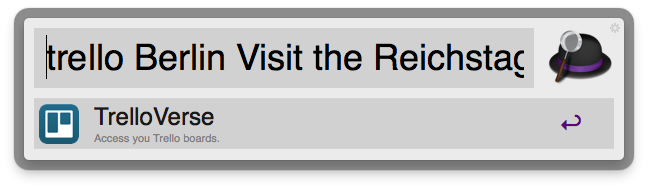
\includegraphics[width=\textwidth]{figures/trello-ext.png}
\caption{Alfred Extension for Trello: This command would add a card with the name \emph{Visit the Reichstag} to the board called \emph{Berlin}.}
\label{fig:trello-ext}
\end{figure}

If you omit the text after the board name the extension will show you all card names of this board and its statuses.

Sometimes there are several boards with similar board names. In this case the extension will pick the \textquotedblleft last\textquotedblright match. So if you have two boards called \emph{Berlin} and \emph{Berlin sightseeing} the extension will would pick \emph{Berlin sightseeing}. This approach makes sense because if the extension would pick the first match, in this case \emph{Berlin}, it wouldn't be possible to access \emph{Berlin sightseeing}. In the case that one wants to access \emph{Berlin} and add a new card beginning with \emph{sightseeing} one has to put this board name betweet tick marks.

\todo{Code this and verify the practicability.}

\section{Native applications}
Although Trello is an extremely good web-app, I'm of the opinion that a native application is always the better solution. The first reason is because it's a dedicated app and so it's integrated with the operationg system. Especially for todo-applications it's an advantage that they can access the systems notification system, or that they could completely vanish in the background so they don't bother the user while working. There are mobile applications for iOS \cite{trello:ios} and Android \cite{trello:android} by Trello itself. But theres no Mac, Windows or Linux application.

A native application would even speed up the Alfred extension because the application could cache the data. So there hasn't to be an actual HTTP request for every command by the Alfred extension. And if a HTTP request necessary the user hasn't to wait because the application will handle the command in the background.
\cleardoublepage


%%%%%%%%%%%%%%%%%%%%%%%%%%%%%%%%%%%%%%%%%%%%%%%%%%%%%%%%%%%%%%%%%%%%%%%%%%%%%
%%% Bibliographie
%%%%%%%%%%%%%%%%%%%%%%%%%%%%%%%%%%%%%%%%%%%%%%%%%%%%%%%%%%%%%%%%%%%%%%%%%%%%%

\addcontentsline{toc}{chapter}{Bibliography}

\bibliographystyle{alpha}
\bibliography{mylit}
%% Obige Anweisung legt fest, dass BibTeX-Datei `mylit.bib' verwendet
%% wird. Hier koennen mehrere Dateinamen mit Kommata getrennt aufgelistet
%% werden.

\cleardoublepage

%%%%%%%%%%%%%%%%%%%%%%%%%%%%%%%%%%%%%%%%%%%%%%%%%%%%%%%%%%%%%%%%%%%%%%%%%%%%%
%%% Erklaerung
%%%%%%%%%%%%%%%%%%%%%%%%%%%%%%%%%%%%%%%%%%%%%%%%%%%%%%%%%%%%%%%%%%%%%%%%%%%%%
\thispagestyle{empty}
\section*{Selbst\"andigkeitserkl\"arung}

Hiermit versichere ich, dass ich die vorliegende Diplomarbeit 
selbst\"andig und nur mit den angegebenen Hilfsmitteln angefertigt habe und dass alle Stellen, die dem Wortlaut oder dem 
Sinne nach anderen Werken entnommen sind, durch Angaben von Quellen als 
Entlehnung kenntlich gemacht worden sind. 
Diese Diplomarbeit wurde in gleicher oder \"ahnlicher Form in keinem anderen 
Studiengang als Pr\"ufungsleistung vorgelegt. 

\vskip 3cm

Ort, Datum	\hfill Unterschrift \hfill 
%%%%%%%%%%%%%%%%%%%%%%%%%%%%%%%%%%%%%%%%%%%%%%%%%%%%%%%%%%%%%%%%%%%%%%%%%%%%%
%%% Ende
%%%%%%%%%%%%%%%%%%%%%%%%%%%%%%%%%%%%%%%%%%%%%%%%%%%%%%%%%%%%%%%%%%%%%%%%%%%%%

\end{document}

